% project proposal
\documentclass[12pt,a4paper]{article}
\usepackage{times}
\usepackage{setspace}
\usepackage{cite}
\usepackage{url}
\usepackage{harvard}
\usepackage{lipsum}
\usepackage{color, soul}
\usepackage{amsmath}
\usepackage{float}
\usepackage{graphicx}
\graphicspath{ {./images/} }


\floatstyle{boxed}
\newfloat{code}{h}{lop}
\floatname{code}{Code}


\title{Computing Project\\UFCE3B-40-3\\Project Draft}
\author{Neil Donnelly\\10032122\\
\texttt{neil.m.donnelly@gmail.com}
}
\date{\today}

% title page
\begin{document}
\maketitle
\thispagestyle{empty}

\begin{quote}
    \begin{center}\Large Exploiting Multi-Core Processors through Functional Programming
    \end{center}
\end{quote}
    \begin{center}
        {\fontsize{50}{60}\selectfont $\lambda$}
    \end{center}
\newpage

% acknowlegements
\doublespacing
\pagestyle{empty}

\vspace*{\fill}
    \begin{center}
        \Large Acknowledgements \\
        \large
        To Ron Burgundy\ldots You stay classy\\
    \end{center}
\vspace*{\fill}
\newpage

% abstract page
\begin{abstract}
\lipsum[1-2]
\end{abstract}
\newpage

% contents page
\pagestyle{plain}
\pagenumbering{roman}
\setcounter{page}{1}
\tableofcontents

\newpage

% start of text
\pagestyle{plain}
\pagenumbering{arabic}
\setcounter{page}{1}

\doublespacing
% start introduction of report

% set the citation style to dcu and the connector to &
\citationstyle{dcu}
\renewcommand{\harvardand}{\&}

\section{Introduction}
\subsection{Context}
\subsubsection{Moore's Law}

In 1965, George Moore observed that the number of components which can be deployed onto a semiconductor integrated circuit, or `chip' appeared to be exponentially doubling every year \cite{fiftyYearsOfMoores}. Moore conjectured that this trend would continue for the proceeding ten years; with increasing chip area, decreasing feature size and improved circuit designs \cite{endOfSemiconductors}.

Moore did not however, observe that such rapid growth is infinitely sustainable, and predicted a decline in the rate of exponential growth to a doubling of components over a more sobering two year interval \cite{fiftyYearsOfMoores}.

This observation is known as Moore's law, and drives semiconductor development with the inevitability of a self-fulfilling prophecy. Indeed, development out paces the law, resulting in a doubling of components in cycles of circa 18 months \cite{fiftyYearsOfMoores}.

\subsubsection{The Benefits of Moore's Prophecy} 

The dramatic increases in semiconductor development result in chips which are cheaper, lighter, faster, less power hungry and more reliable than their predecessors \cite{fiftyYearsOfMoores}. This almost mystical effect of Moore's law on the semiconductor industry allows for \cite{fiftyYearsOfMoores}  \textit{`a life without tradeoffs'}, in which the cost of producing chip components continues to reduce along with their size. The net result being an almost constant production cost for manufacturers and an environment in which further chip development appears to be protected from traditional economic factors \cite{fiftyYearsOfMoores}.

The cumulative effect of exponential gains gives present day chips incredible power and complexity, which both underpin the continued growth of the software industry and facilitate an inevitability of ubiquitous computing. Indeed, many processing intensive applications which are taken for granted, such as high definition video would be inconceivable without the exponential performance gains of which Moore's Law professes \cite{theKillRule}.

\subsubsection{Moore's Gap}

Unfortunately, whilst `The Law' continues unabated, the level of performance which can be wrung from any given chip is beginning to decrease \cite{theKillRule}. This gap between the law's continued proliferation of micro architecture and the real world performance gains follows Pollock's Law \cite{thousandCoreChips}, which states that doubling the logic of a processor core results in performance gains of a mere 40\%.

Pollocks Law is further compounded by what is proving to be an end to Chris Mack's \textit{`no tradeoff'} era \cite{fiftyYearsOfMoores}. The faster, smaller, less power hungry transistors rely upon voltages scaling down along with their size \cite{frequencyAndVoltage}. Unfortunately, with the laws of physics being less than accommodating in this regard; this is not currently possible \cite{frequencyAndVoltage}. The net result is that the designers are unable to furnish the world with the ever increasing clock speeds to which it is accustomed. This \textit{`Moore's Gap'} \cite{theKillRule} requires that chip designers implement new chip architectures in order to circumvent the immense power demands and thermal output which are the consequence of complex, high frequency cores \cite{frequencyAndVoltage}.

\subsubsection{A New Breed of Processor}

In order to bridge the expanding gap between Moore's Law and real world performance; manufacturers turn their focus from producing chips which sport massively powerful single cores to the development of `multi-core' processors \cite{thousandCoreChips,frequencyAndVoltage}. This new breed of chip comprises several processing cores, which run at lower clock speeds; the net result being that the aforementioned power and thermal constraints are conveniently sidestepped when implemented with an adequate frequency and power management scheme \cite{frequencyAndVoltage}.

Unfortunately however, it is hypothesised \cite{thousandCoreChips} that continuation of multi-core development again results in unfeasible power demands, which are again attributed to the issue of voltage scaling. It is estimated that a single chip built upon a 300mm$^{2}$ processor die will require around 1000 watts of power in order to operate \cite{thousandCoreChips}.

It is therefore proposed that development of new `many-core' processing architectures which are able to provide a panacea to the issues of voltage scaling \cite{thousandCoreChips}. The many-core architecture is similar to that of multi-core, with a significant reduction in core complexity and proliferation in the number of cores on any given chip. The result is a processor comprised of a plethora of much simpler cores, which being mindful of Pollock's Law allows for processors with the highest possible performance to complexity ratio \cite{thousandCoreChips}.

\subsubsection{A New Breed of Problem}

In 1967, Gene Amdahl addressed the AFIPS Spring Joint Computer Conference \cite{amdahl}. He argued in favour of more powerful single cores; stating that for the vast majority of cases only a fraction of a program's code could be effectively parallelized \cite{amdahl}. Amdahl's observations, simply put, state that the performance gains from a multi-processor or multi-core architecture are limited by the volume of serial code which is present in any given system. \cite{thousandCoreChips}.

A re-evaluation of Amdahl's Law \cite{reevaluateAmdahl} suggests that the initial observations regarding the volume of system code which can be parallelized may be misleading. Gustafson \cite{reevaluateAmdahl} conjectures that Amdahl's Law does not account for the problem size scaling with the available processing power, and that it is natural for software engineers to take advantage of new hardware in previously unforeseen ways. This hypothesis is further supported by Hill \& Marty \cite{amdahlsLawMultiCore}; who postulate that a reconciliation between Amdahl's observation and Gustafson's re-evaluation is required in order for the continued exploitation of Moore's Law. Unfortunately, there is no perfect solution to draw upon. The current consensus however, is that it is imperative for software engineers to begin to find ways in which to parallelize increasingly greater percentages of any given system in order to harness the maximum amount of available processing power \cite{reevaluateAmdahl,thousandCoreChips,amdahlsLawMultiCore}.

Herb Sutter \cite{theFreeLunchIsOver} recalls a pattern of chip and software development, which through the 1990's is known as \textit{``Andy giveth, and Bill taketh away"}. This refers to the performance gains created by Intel's chips and the subsequent, almost inevitable expansion of the latest Windows release to consume the benefits thereof. This phenomenon however, is not exclusive to software created by the Microsoft corporation; but has perpetuated itself over the lifespan of the software industry \cite{theFreeLunchIsOver}. In what appears to be software development's interpretation of Parkinson's Law \cite{parkinsonsLaw}, increases in chip throughput are rarely treated with a high level of delicacy \cite{theFreeLunchIsOver}. The result is software which appears to expand over the available resources in an almost effortless manner.

This laissez-faire attitude towards development stems from the knowledge that no matter how inefficient a software product may be; within 18 - 24 months such inefficiency will be counterposed by further increased core speeds \cite{theFreeLunchIsOver}. However, in a similar manner to which Chris Mack's \textit{`no tradeoff'} era no longer applies to chip development \cite{fiftyYearsOfMoores}, this \textit{`free lunch'} for software developers appears to have reached its terminus \cite{theFreeLunchIsOver}. Indeed, with it being suggested that more cores and lower speeds are the way in which to bridge Moore's Gap; many vendors could begin to see the performance of their products diminish significantly on newer hardware \cite{theFreeLunchIsOver,concurrencyChallenges}.

In response, a different approach is required \cite{concurrencyChallenges}. Creating safe, threaded software for anything other than a trivial application is demanding, difficult and expensive \cite{concurrencyChallenges}. With the future being multi-core, it appears that the software industry should seek to adapt to this new parallel world if it is to continue to advance. Somewhat interestingly, a paradigm which may facilitate this brave new world of parallel development was first published in the 1930's, implemented in the 1950's and is subject to further refinement \cite{church1936,lispPart1,joyOfClojure}. It is known as functional programming, and could potentially aid in the production of safe concurrent software \cite{promisesOfFunctionalProgramming}.

\subsubsection{Language Selection}

In all endeavours it is important to use the correct tool for the job at hand. Selection of a programming language will influence factors such as the effort required to complete the code, its runtime efficiency, memory usage, reliability and portability \cite{languageComparison}. Conveniently, the ease at which robust concurrent systems may be produced is also influenced by the implementation language \cite{paraFuncImp,promisesOfFunctionalProgramming}.

In 1989 Peyton Jones \cite{paraFuncImp} postulated that functional programming is inherently suited towards the production of parallel systems. The conclusion reached is an expectation that functional programming and parallelism will begin to find more widespread use \cite{paraFuncImp}. More recently, the realisation that the industry requires tools more suited to developing concurrent code is gaining further acceptance \cite{promisesOfFunctionalProgramming}. The purported benefits of these tools must therefore be investigated in order to determine if they are worthwhile ventures.


\subsection{Research Question}

To what extent can functional programming exploit the potential performance gains of multi-core processors? 

%Start Background of report BACKGROUND
\newpage
\section{Background}

In order to fully grasp the implications of utilising a functional language, it would first serve to define in as exact terms as possible what a functional language is, and what distinguishes one from its imperative counterparts. 

To this end, the reader is presented with a simplified introduction to the mathematical model upon which functional programming is based. Following this, and with the intention of further crystallizing the definition of what it means to program in a functional manner, the first true functional language LISP is presented. Finally for functional programming, the language conceived with the express purpose of approaching concurrent programming is presented; the reader learns about Clojure.

With a newfound understanding of functional programming, it is now that the challenges of writing parallel programs are examined alongside the current state of the art industry best practices, which attempt to manage concurrency and stop it getting out of hand.

Finally, the suitability of applying Clojure to the aforementioned challenges is investigated.

\subsection{Programming Languages}

\subsubsection{Imperative Programming}

The overwhelming majority of programs in execution today are written in imperative programming languages. An imperative language can be said to have had its method of computation derived from Alan Turing's Universal Turing Machine \cite{turing1936,ImperativeFunctional}; and has been loosely defined as a language \textit{``where a sequence of statements mutates program state"} \cite{joyOfClojure}. It is assumed that the reader of this document is experienced with at least one imperative language such as Java, C, Ruby, Python\ldots etc. As such, it is determined that further explanation of the imperative paradigm is unnecessary, as it is well understood by the computing community in general.

\subsubsection{Functional Programming}

Fogus \& Houser postulate that functional programming is a difficult term to accurately define, as any given definition will be biased towards the specific functional language used by the individual in question. They continue, stating that even within academia it can often be contradicted from one paper to the next \cite{joyOfClojure}. For a field in which precise definitions are foundational; an inconsistent view of what constitutes functional programming is a formidable issue to be sure. Fortunately however, Fogus \& Houser provide a definition which covers the core tenets of functional programming regardless of language or viewpoint:
\begin{quote}
``Functional programming concerns and facilitates the application and composition of functions. Further, for a language to be considered functional, its notion of function must be \textit{first class}. The functions of a language must be able to be stored, passed and returned just like any other piece of data within that language." \cite{joyOfClojure}
\end{quote}

With this definition as a starting point it is possible to see the how the LISP family of functional languages were derived from Alonso Church's untyped lambda ($\lambda$) calculus \cite{church1936,lispPart1}. It would therefore be beneficial to first discuss and understand some basic principals of $\lambda$ calculus before considering the features of specific functional languages.

%LAMBDA
\subsubsection{$\lambda$}

In 1932 Alonso Church published a paper detailing a formal model of computational expression \cite{church1932}. The model is an extension of studies conducted into mathematical functions by Frege in 1893, and was created with the intent to allow the proof of computations by methods of substitution and variable binding \cite{lambdaHighlights}. Unfortunately, the paper and the method within were proved inconsistent when subjected to further investigation \cite{lambdaHighlights}.

Unperturbed, Church returned in 1936 with a paper proving the impossibility of the Entscheidungsproblem \cite{church1936,churchTuringThesis}. He achieved this using a refined and much stronger model of computation; the untyped $\lambda$ calculus \cite{church1936}. Independent of Church's work, Alan Turing also addressed the Entscheidungsproblem, reaching the same conclusion through the computational method of his Universal Turing Machine \cite{turing1936,churchTuringThesis}.

It is further observed that the computational processes of untyped $\lambda$ calculus and Alan Turing's machine are equivalent in the types of functions which they are able to express. This parity between the two calculation methods is formalised as the Church-Turing Thesis \cite{churchTuringThesis,ImperativeFunctional}.

\subsubsection{$\lambda$ Notation \& Evaluation}

As stated, $\lambda$ calculus works by resolving the values of a function or program by a method of substitution. It consists of what would appear to be limited syntax and expressive potential; however is powerful enough to represent all computable functions \cite{church1936}. The syntax is defined below in Backus-Naur form \cite{bnf}.

\begin{quote}
    {$<expression> \mbox{ := }  <name> | <function> | <application>$}
    {$<function> \mbox{ := } \lambda <name>.<expression>$}\newline
    {$<application> \mbox{ := } <expression><expression> $}\newline
\end{quote}

The language allows the definition of three different $\lambda$ expressions: names of variables, function definitions and the application of function definitions to either variables, other function definitions or other applications.

A $\lambda$ function (also known as an abstraction) is a representation of an anonymous function, which defines the \emph{name} to the left of the '.' operator as an argument, with the \emph{expression} on the right being the return value \cite{church1936}. Hence the function $\lambda x.x$ would be a function which returns the supplied argument. As functions and names are both expressions, this means that $\lambda$ calculus allows functions to be both supplied as arguments to and returned from other functions \cite{church1936}.

Expressions in $\lambda$ calculus are evaluated by applying the function on the left to the expression on the right. Parenthesis are used in order to make explicit the order of application. For example, this series of expressions:
\begin{displaymath}
    \lambda x.x \lambda y.y \lambda z.z
\end{displaymath}
Could parenthesise to:
\begin{displaymath}
    (\lambda x.x) ((\lambda y.y) (\lambda z.z))
\end{displaymath}
Or alternatively:
\begin{displaymath}
    ((\lambda x.x) (\lambda y.y)) (\lambda z.z)
\end{displaymath}

At this point, it is imperative to understand the difference between variables which have been bound and variables which are free to assume any value. If a function $\lambda x.y$ is declared, the \emph{name} given to it's argument, in this case $x$, is considered bound within the function's \emph{expression}. The result of this variable scoping is that should we supply an argument to $x$, say $t$:
\begin{displaymath}
    (\lambda x.y)t
\end{displaymath}
Any occurrence of $x$ within the function body $y$ will have the same value as the parameter bound to the $\lambda$ symbol. In this case, the value of $\lambda x$ is $t$. In contrast, $y$ is a variable free to take on any value, as it does not exist within an expression in which $y$ has been bound to a $\lambda$. This distinction between free and bound variables allows for the same name to be used several times but exist with different values depending on its scope.

The binding of variables to the $\lambda$ operator introduces an important functional aspect known as a closure; in which any functions nested within the body of another function will use the parent function's bound variable. For example:

\begin{displaymath}
    ( \lambda x.(\lambda y.xy)y)x
\end{displaymath}

Here we have a function which takes the far right argument $x$ and binds it to $\lambda x$. The body of $\lambda x$ consists of another function which takes the value of $y$, binds it to $\lambda y$ and then returns the value of applying $x$ to $y$. Due to the closure, the value of $x$ in $\lambda y$ is the same as that bound to $\lambda x$.

Somewhat interestingly, $\lambda$ calculus only allows the definition of functions which accept a single argument. In order to evaluate multiple arguments, a technique called currying is employed. This consists of creating a function which accepts the first argument. The function then returns another function which will accept the second argument. This continues until such a point that a function is produced which returns a variable or value. Currying is made possible by the use of closures, as bound variables remain bound even within nested functions which are returned. If a function definition which accepts three variables $x,y,z$ and returns another variable $r$ is considered; its curried notation would be:
\begin{displaymath}
    \lambda x. \lambda y. \lambda z.r
\end{displaymath}
In order to invoke the function it must be supplied with three expressions (arguments):
\begin{displaymath}
    (((\lambda x. \lambda y. \lambda z.r) t ) u ) v
\end{displaymath}
In this, $t$ is supplied to $\lambda x$, $u$ to $\lambda y$ and $v$ to $\lambda z$. Due to the scoping and binding of variables, it is then possible to create a function which adds two numbers together, supplied with the arguments 5 and 6:
\begin{displaymath}
    ((\lambda x. \lambda y.(x+y) ) 5 ) 6
\end{displaymath}

Applications in $\lambda$ are resolved via a method called $\beta$ reduction, which attempts to produce the simplest possible answer by recursively replacing function definitions with the values of their computations. Take the $\lambda$ application:
\begin{displaymath}
    (\lambda x.x)5
\end{displaymath}
Which reduces to:
\begin{displaymath}
    5
\end{displaymath}
More complicated functions can be reduced in a series of steps:
\begin{align*}
    & (((\lambda x. \lambda y. \lambda z.(x + y + z))3)4)5 \\
    & ((\lambda y. \lambda z.(3  + y + z)4)5 \\
    & (\lambda z.(3 + 4 + z)5 \\
    & 12
\end{align*}

$\lambda$ calculus introduces some important concepts to the field. The notion of using the substitution method through pure functions which have no side effects\footnote{Functions do not modify any state and are consistent when given the same inputs \cite{sideEffects}.}, allows for the definition of programs which can be completely deterministic and mathematically tractable. Because of this tractability, functions can safely be treated as first class citizens, used as arguments and returned from other functions. If Fogus \& Howser's definition of functional programming is considered, then $\lambda$ calculus would indeed appear to be genesis. 

%LISP
\subsubsection{LISP}

List Processing, or LISP was developed by John McCarthy between 1956 and 1960. LISP was born from the fundamentals of $\lambda$ calculus and the first attempt at an artificial intelligence centric language called \emph{Information Processing Language} \cite{lispPart1,historyOfLisp}. It is considered high level and is the first programming language to implement garbage collection, recursion and a complete if-then-else statement \cite{lispPart1,historyOfLisp,beatingTheAverages}.

Its form is instantly recognisable from the use of parenthesis to define expressions \textit{e.g. Code~\ref{code:lisp}} and its use of polish prefix notation \cite{historyOfLisp} in which the operand or function is applied to all proceeding elements; as in the example \textit{Code~\ref{code:lisp2}} from Abelson \& Sussman \cite{structureAndInterpretation}.
\begin{code}
  \begin{verbatim}

(+ (* 3
      (+ (* 2 4)
         (+ 3 5)))
   (+ (- 10 7)
      6))
  \end{verbatim}
  \caption{Parenthesised LISP with prefixed operands}
  \label{code:lisp}
\end{code}

\begin{code}
  \begin{verbatim}

(+ 21 35 12 7)
= 75

(* 25 4 12)
= 1200
  \end{verbatim}
  \caption{Polish prefix notation resolution}
  \label{code:lisp2}
\end{code}

All data within a LISP program is either of two data types, an atom or a list. A list is a sequence of elements, each element of which is itself either an atom or a list. Whereas an atom is either a number or a symbol. Lists themselves consist of primitive pairs that act as building blocks for more complex structures \cite{lispPart1,structureAndInterpretation}.

\begin{figure}[h]
  \centering
  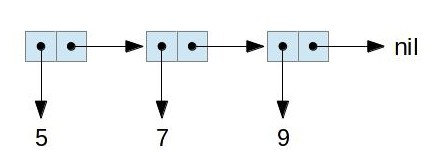
\includegraphics[scale=.5]{list}
  \caption{Lists and Atoms}
  \label{fig:listsAndAtoms}
\end{figure}

The above list in \textit{Figure~\ref{fig:listsAndAtoms}} is represented in \textit{``box-and-pointer notation"} \cite{structureAndInterpretation} and  would evaluate to a list of the numbers: $[5, 7, 9]$. Each element consists of two pointers, which point to either an atom or a list. It is perhaps not immediately apparent, however using this simple method of structuring data it is possible to model complex items \textit{Figure~\ref{fig:listsAndAtoms2}}.

\begin{figure}[h]
  \centering
  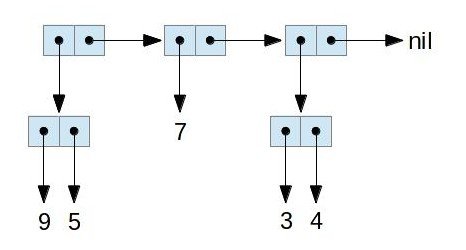
\includegraphics[scale=.5]{list2}
  \caption{A more complex list structure}
  \label{fig:listsAndAtoms2}
\end{figure}

A LISP program consists of symbolic expressions (or S-expressions). These expressions are evaluated and converted into the aforementioned list structures which then reside in memory \cite{lispPart1,historyOfLisp}. Thus the textual code written in the example \textit{Code~\ref{code:lispInText}} is interpreted into an actual data structure shown in \textit{Figure~\ref{fig:codeAsData}} \cite{structureAndInterpretation}.

\begin{code}
  \begin{verbatim}

(+ (* 3 3) 4)
  \end{verbatim}
  \caption{LISP as written in editor}
  \label{code:lispInText}
\end{code}

\begin{figure}[h]
  \centering
  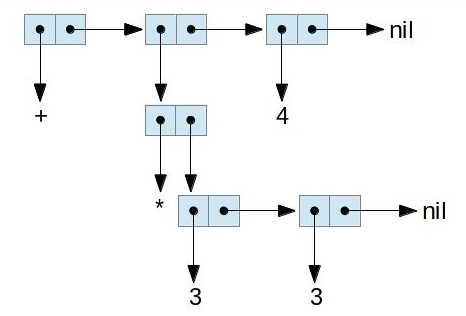
\includegraphics[scale=.5]{codeAsData}
  \caption{LISP code as a data structure}
  \label{fig:codeAsData}
\end{figure}

The inherent power of this method of interpretation is that the code written in the text editor now exists in a form which can be manipulated at run time \cite{lispPart1}. Code is stored in the same manner as data, is just as malleable and can be passed around the program in the same way. This allows the LISP programmer to utilize a powerful language construct called a macro to create, as George Graham stated \textit{``programs that write programs"} \cite{beatingTheAverages}.

The original LISP specification consists of a mere seven functions and two special forms. Like the $\lambda$ calculus it manages to describe \textit{``the whole of computation"} \cite{joyOfClojure} using a minimalistic and elegant syntax \cite{lispPart1}. It is considered by some to still be amongst the most the most powerful languages available, regardless of it's lack of widespread commercial use \cite{beatingTheAverages,joyOfClojure}.

\subsubsection{Clojure}

Clojure is a response to a perceived need. The 

\subsection{Concurrency}

\begin{quote}
  \textbf{Con $\cdot$ cur $\cdot$ rent} \\
  1. Occurring or existing simultaneously or side by side \ldots\\
  \cite{concurrentDef}
\end{quote}

Concurrency effectively means that things happen at the same time. When speaking of concurrency in relation to software development, one of two processes are occurring:

\begin{enumerate} \itemsep0pt
        \item \textbf{Simulated concurrency:} The host platform has a single processor; therefore threads and processes are interleaved and are scheduled to use the processor at different intervals. This affords an illusion of simultaneous execution.
        \item \textbf{Simultaneous execution:} The host platform has multiple processors or processor cores and can execute threads and processes simultaneously.
\end{enumerate}
Regardless of the process which is in occurrence, once a developer decides to use threads or multiple processes, the net result is the same and concurrency becomes a very real issue and concern. The prime directive of the concurrent developer is to not allow the system to produce inconsistent data; that is to ensure that all related data  \cite{javaConcurrency}.

\subsubsection{State and Mutability}

Any discussion regarding the issues related to concurrency almost inevitably leads to the consideration of both state and mutability.

\begin{quote}
    ``An object is said to ``have state" if its behaviour is influenced by its history." \cite{structureAndInterpretation}
\end{quote}

The seminal book; Structure and Interpretation of Computer Programs \cite{structureAndInterpretation} is the companion text for class 6.001 at the Massachusetts Institute of Technology. Between the years of 1980 and 2008, class 6.001 fulfils the role of introducing first year students to programming and software engineering at one of the leading institutions for technological research and computer science.

What's interesting about the text is that it patiently waits until page 217 before approaching the matters of state, modularity and objects \cite{structureAndInterpretation}. Prior to page 217, students are instead introduced to concepts such as expressions, linear recursion, tree recursion, iteration and data abstraction. Indeed, the first appearance of an assignment operator occurs on page 220, with almost 50\% of the book having elapsed \cite{structureAndInterpretation}.

In contrast, if compared to a recommended text for programming 101 at another institution, for instance: Learning Java \cite{learningJava}. It is found that the first appearance of the assignment operator is on page 31; the related heading of Instance Variables being only 12 pages further ahead \cite{learningJava}.

Why then, given that assignment and state are fundamental to producing meaningful systems \cite{structureAndInterpretation} is there such a delay regarding this particular discussion? Thankfully, Abelson and Sussman are not beyond detailing their motives.

\begin{quote}
    ``With objects, we must be concerned with how a computational object can change and yet maintain its identity. This will force us to abandon our old substitution model of computation in favour of a more mechanistic but less theoretically tractable \textit{environmental model} of computation." \cite{structureAndInterpretation}
\end{quote}

It would appear that the addition of the assignment operator and the concept of mutable state is of concern to the authors. With the results of their functions becoming less mathematically defined and more unpredictable, they have reached the somewhat counter-intuitive conclusion that assignment is in fact a more complex subject to comprehend than recursion \cite{structureAndInterpretation}. A conclusion which the vast majority of first year computing students would, most likely, emphatically refute. They elaborate further, detailing the primary culprit of this increased complexity.

\begin{quote}
    ``The difficulties of dealing with objects, change, and identity are a fundamental consequence of the need to grapple with time in our computational models. Those difficulties become even greater when we allow the concurrent execution of programs." \cite{structureAndInterpretation}
\end{quote}

If then, a root cause of concurrent programming challenges is sought, the industry need look no further than change over time, or mutability. Rich Hickey postulates that when developing using mutable objects, the state of the resulting system becomes difficult to both predict, replicate and test \cite{areWeThereYet}. The issue is further compounded when interconnected mutable objects are introduced to multiple threads and the developer must now deal with the inherent issue of non-determinism which concurrency introduces \cite{concurrencyChallenges}.

The issue of controlling the identity of an object over time is not something revelatory, however something which is currently accepted and understood as a challenge of computer science. It is however an issue which has been brought to the fore now that processing power is becoming increasingly parallelized \cite{concurrencyChallenges,theConcurrencyChallenge}.

\subsubsection{Race Conditions}

Consider the flow of execution in \textit{Figure~\ref{fig:concurrentProblem}}.
\begin{figure}[h]
  \centering
  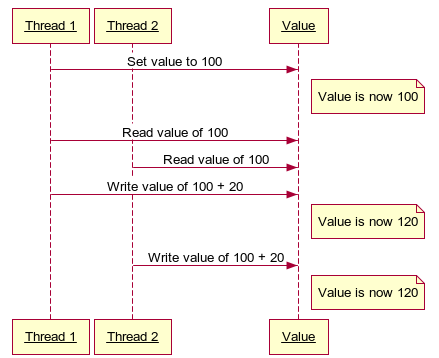
\includegraphics[scale=.65]{raceConditions1}
  \caption{Race conditions on mutable data}
  \label{fig:concurrentProblem}
\end{figure}
Two threads both wish to increment a mutable variable by 20 each. The variable in question is initially set to have a value of 100. The expectation therefore is that the variable's value will be 140 when both threads have finished. Unfortunately, as threads introduce a non-deterministic outcome to a program's execution it's entirely possible that the outcome will be that of \textit{Figure~\ref{fig:concurrentProblem}}; whereby both threads read a value of 100, rather than the first thread reading a value of 100 and the second reading a value of 120. The result of these operations is inconsistent and makes the system in which it resides completely probabilistic and thus difficult to understand.

The nature of concurrent execution means that the developer can never be sure which thread of execution will get to a variable first, or indeed if a thread will be able to both read and write the data before another thread also reads and writes the data. These \emph{race conditions} require a good strategy in order to be well marshalled.

\subsubsection{Deadlock}
Deadlock occurs when two or more threads obtain exclusive locks for specific shared resources and then each require access to the resources the other has locked. 

In \textit{Figure~\ref{fig:deadlock1}} it is demonstrated that thread 1 gains access to resource A and thread 2 gains access to resource B. In order to continue operation, thread 1 also requires resource B and thread 2 requires resource A. With both resources already being locked, both threads will sit in limbo awaiting the release of a resource which will never happen. Both threads are blocked and now completely useless.
\begin{figure}[h]
  \centering
  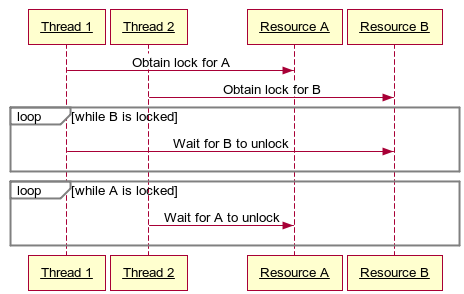
\includegraphics[scale=.65]{deadlock1}
  \caption{Deadlock of two threads}
  \label{fig:deadlock1}
\end{figure}

\subsection{Concurrent Strategies}

In order to effectively control mutability, the industry has developed several strategies which allow the management of concurrently accessible mutable data \cite{javaConcurrency}. Unfortunately, even the best sources of concurrent strategies concede that this is an area which is very difficult to get right, and that if data were immutable the development of concurrent systems would be much easier \cite{javaConcurrency,theConcurrencyChallenge}. That being said, let's examine some current best practices for concurrent software development.

\subsubsection{Locking}

If a developer requires that a resource needs to be safe from inconsistent reads and writes they can lock the aforementioned area. This allows a single thread to obtain the key to the resource and gain exclusive access to that particular piece of code. The side effect of locking is that all other threads which also need access to the locked area are now blocked and must wait until they have sole ownership of the key before proceeding \cite{javaConcurrency}.

This appears to be a sound idea in principal; however there are some issues with locks; especially for multiple stage operations.

Firstly, locking is a convention or an agreement, which is adhered to by software developers and is not typically enforced by any mechanistic means. This becomes a large issue, as not every resource a developer uses needs to be locked. It introduces a fallible component (namely a human) into the system, as the developer must keep track of which resources need to be locked and which can be used without locks. Additionally, should a decision be made to lock a previously unlocked resource, all locks must be retrofitted to existing code, again by fallible human means.

Locks also introduce bottlenecks into the system. As one thread gains access to a particular resource all other threads requiring the resource are now blocked, unable to continue their execution until such a time that they can get hold of the key. This is an issue on single core machines, but on a multi-core machine the net result is a massive waste of processing power \cite{theConcurrencyChallenge}.

Before continuing it would be useful to define two groups which wish to access shared resources: readers and writers. Readers, as you would expect require read only access to a particular resource and will not introduce inconsistent data to a system, whereas writers require both read and write access and could potentially cause data integrity issues if left unchecked.

If a typical lock is considered, then when a reader has a key it blocks all other readers from accessing the same resource. This is blatantly inefficient as locks exist to protect data integrity from writes. Therefore readers need not block other readers from accessing a resource which they are not going to change \cite{javaConcurrency}.

The solution to this particular issue is the use of a more complex lock which allows multiple readers to access a resource, but only a single writer. This is a much improved strategy, however still introduces the blocking aspect during writes.

There are two basic locking strategies which can be used, each with their own trade offs and considerations.

\subsubsection{Coarse Granularity Locking}

In terms of parallel programming complexity managing a single resource with locks is child's play. Unfortunately, in the real world operations are performed on multiple resources by multiple threads and can require several locks at any given time. This introduces deadlock as previously described \cite{javaConcurrency}.

A strategy to deal with this is coarse granularity locking. This implies that a number of resources are obtained for a thread's exclusive use with a single lock. This is simple to both describe and document, and is considered to be one of the safest locking schemes for multiple resources (providing that each resource only appears in a single lock).

Naturally, there is a trade off for such ease of use, namely throughput. Coarse granularity locking instantly makes any resources included in the lock blocking whether the thread which has obtained the lock actually requires them or not. 

\subsubsection{Fine Granularity Locking}

If throughput is of concern when locking resources then fine granularity locking is an effective strategy to utilize. With fine granularity, each critical resource has its own lock. The key to a workable fine granularity locking is to effectively determine a locking strategy which all developers can follow. Failure to do so will likely result in deadlock \cite{javaConcurrency}.

Achieving a workable and consistent locking strategy for the order of obtaining locks is difficult, as all systems are subject to changes. New resources will be added, new locks implemented and the developers must spend considerable effort to maintain the integrity of the locking order.

\subsubsection{Copy On Write Collections}

Useful for when multiple threads are operating on a collection. Within a copy on write collection, if any changes are made to the data within, a copy of the collection is made. This copy is then atomically swapped for the previous version of the collection in a single operation. The net effect of this is that any reads of the collection will result in the reader being presented with a copy of the collection data that will never change. This allows the use of collections which are completely non-blocking \cite{javaConcurrency}.

Unfortunately, copy on write collections still have their limitations. In terms of performance, the write operation is computationally expensive as the collection data is being copied in it's entirety. Copy on write collections perform admirably when used mainly for reading with occasional writes; however do not stand up well to excessive write operations \cite{javaConcurrency}.

Furthermore, operations comprised of multiple steps still require a lock, as copy on write still allows for race conditions if multiple read/write steps are required from separate concurrent operations \cite{javaConcurrency}.

\subsection{Clojure's Concurrent features}

--- concurrency methods ---
conventional way -- direct references to things that can change - soon as you do it you're stuck with it. lock n' hope for best - manual - all decided by convention - not in programming language, convention is outside of the program - bad.


--- clojure ---
must feel that things are changing sometimes - keep the reference, but the reference can mutate, indirect. indirect references to things which never change. can change the reference atomically refFred - at one point in program it refers to one thing, later refers to something else. don't really have a pointer to the structure, have a referemce. references are mutable, only thing which can change - ref types - they have concurrency semantics. must use functions to make them point to diff things via functions, enforced and automatic. 

-- from convention -- to enforcement --

-- no locks! --
-- three refs in clojure --
-- var= global values, can also be bound inside other threads - for isolating changes in threads. changes in threads will not cut across to other threads - like special variables in common lisp with thread semantics - stack discipline, will unwind to their initial state

-- refs= transactional structure, co-ordinated changes, can be seen from multiple threads. refs make changes which can be seen from multiple threads vis transactions atomic
-- software transactional memory system -- application level -- ref can only be changed in transaction, change is atomic and isolated. all changes make to set of refs in transaction - or none - isolated, you don't see the effects of other transactions and they don't see yours till commit -- speculative and automatically retried. transactions will rety so you can be second when attempting transactions. therefore transactions cannot have side effects. refs only manipulated in transactions. All changes appear to happen at the same point in time. there is no staggering of changes. -- consistent view of the entire world - readers never block writers, writers never block readers.


--agents= make requests for something to change, will do so in it's own time eventually; other threads can see the changes. agents are like workers, refs are like
-- manager independant state - agent is responsible for state - you send the agent an action, which says apply this function to whatever state you have inside of yourself.
- you send actions to agents, the request gets queued up in the agent, and eventually this will eventually happen. high degree of independant. you can request, immediately continue and the request will change eventually. one action per agent serialised by the system. none-blocking. things happen in order -- state is always available, can access it. may not reflect all actions which have been sent to it, but not having to wait is awesome. can make sure the work is done with a wait - so will block. - agent can send actions to other agents, will happen in order - agents can co-operate with transactions, can dispatch action within transaction, will only be sent when it commits, so can tie a side effect.

-- lock the world and give me a valid report -- consistency valuable  -- enforced consistency

\cite{promisesOfFunctionalProgramming}
\cite{theFreeLunchIsOver}
\cite{concurrencyChallenges}

\newpage
\subsection{GPGPU}

When speaking of processors and processing throughput it is becoming somewhat impossible to ignore the impact of GPGPU upon massively parallelized algorithms \cite{gpuTutorial}.

\subsubsection{What is GPGPU}

GPGPU, short for general-purpose computing on graphics processing units is the act of utilizing the processing unit of a computer's graphics card in order to perform computations. Modern graphics cards have a many core architecture comprised of several hundred small processing cores which share the graphic card's memory \cite{gpuTutorial}. 

When speaking of GPGPU, most sources refer to nVidia's CUDA library and architecture which is exposed through either the use of native C code or via a series of libraries which are available in Java, C\# and other mainstream programming languages \cite{gpuTutorial}.

GPGPU is currently subject to widespread interest and applicative research, especially from computer scientists focused on search \cite{gpuSoftComputing}

\subsubsection{GPGPU Benefits}

In short, GPGPU results in massive throughput, providing that Amdahl's Law \cite{amdahl} is circumvented by a well parallelized algorithm.

In short, and providing that Amdahl's Law is circumvented by a well parallelized algorithm \cite{amdahl}; massive throughput. Speed increases of up to 25x have been recorded on GPGPU when compared to a more traditional processor configuration \cite{gpuMinimisation}.  

\subsubsection{GPGPU Issues}

At the moment, the main issue when considering GPGPU as an option for improving throughput is that of memory latency \cite{gpuTutorial}. As the GPU cannot interface with the main system memory or processor cache, all data must be copied to the GPU's limited internal memory, an expensive operation which wastes clock cycles if performed needlessly \cite{gpuTutorial}.

Perhaps contrary to most other studies performed, Darren Chitty has demonstrated that when cache memory is utilised correctly on multi-core processors, they can garner massive gains in throughput and in some cases outperform the GPU \cite{gpuVsCPU}.

\subsubsection{GPGPU Summary}

It appears that the current GPU has an architecture similar to the proposed many-core processors \cite{thousandCoreChips,gpuTutorial}. As such, they offer incredible throughput \cite{gpuMinimisation}, but offer much more pedestrian memory access speeds \cite{gpuVsCPU}. That being said, they're subject to much current interest and provide an interesting alternative to programming for current CPU's \cite{gpuSoftComputing}.

\subsection{Continuing research}

put links to journals on high speed research here


%HYPOTHESIS
\newpage
\section{Hypothesis}

It is hypothesised that clojure's immutable data structures and transactional assignment allows developers to produce systems which remain consistent over multiple threads of execution. Furthermore, parallel updates to unordered lists offer an opportunity to break down a software problem into much smaller component parts than would otherwise be possible. 

It is therefore postulated that an implementation of a parallel problem in clojure will yield greater performance over the more common imperative languages as the number of system cores increase. It is also the expectation that concurrent programming tasks will take less time to implement, as less time should be spent attempting to debug threaded code. 

%GOALS AND OBJECTIVES
\newpage
\section{Objectives}

This section details the main objectives of the paper along with a list of potential metrics which could be measured implemented in the software product. Also discussed are platform constraints and the extent to which the performance of a platform relates to the performance of a given language.


\subsection{Objectives}

This project sets out to determine if Clojure can to outperform traditional imperative languages and GPGPU when faced with a suitably concurrent problem. To this end, the same case study will be implemented in a number of different languages, whereupon the relative performance of the languages in question will be compared. The following metrics could be measured.

\begin{enumerate} \itemsep0pt
    \item Execution time
    \item Consistency
    \item Memory usage
    \item Production time
\end{enumerate}

It is reasonable to assume that imperative languages easily outperform Clojure in terms of execution time on hardware which has fewer cores. Therefore it would also be useful to determine how many cores are required before Clojure:

\begin{enumerate} \itemsep0pt
    \item Matches the imperative languages for speed.
    \item Begins to assert execution time dominance.
\end{enumerate}

\subsection{Platform and language}

When considering the execution speed of a language, it is likely worth considering the impact which the language platform has on the relative throughput. For instance, Clojure operates atop the Java virtual machine and has many of its features implemented in Java. This adds a level of ambiguity when considering performance; should it be attributed to the language features of Clojure, or to the cleverness of the Java Virtual Machine?

In order to address this ambiguity, it would be useful to include Java in a control group, thus allowing a comparison of pure language features.

\newpage
\section{Requirements Analysis}

To ensure that the objectives of this paper are satisfied, a list of potential features are be drawn up and subsequently prioritised. Following this, a test approach and methodology by which to exercise the test approach are formulated.

Finally, the implementation of the control group is determined along with a suite of acceptance tests

\subsection{Feature List}

In order to correctly prioritise program features and ensure that the most important requirements are satisfied immediately, the MoSCoW method of feature prioritisation is applied to a list of features which would satisfy the defined objectives \cite{moscow}.

\subsubsection{Must}

\begin{itemize} \itemsep0pt
        \item \textbf{Multi-Threaded:} The application uses threads in order to take advantage of multiple CPUS.
        \item \textbf{Shared Data Reads:} The application utilises shared data which is read from by multiple threads.
        \item \textbf{Shared Data Writes:} The application utilises shared data which is written to by multiple threads.
        \item \textbf{Execution Time Logging:} The application can log it's overall execution time and the execution time of individual threads.
        \item \textbf{Implementation in Clojure:} The application will be implemented using the Clojure programming language.
        \item \textbf{Implementation in Java:} The application will be implemented using the Java programming language.
\end{itemize}

\subsubsection{Should}

\begin{itemize} \itemsep0pt
        \item \textbf{Consistency Checking of Shared Data Access:} The application can check its shared data for instances of inconsistent reads/writes.
        \item \textbf{Test Suite:} The application is validated by a suite of unit tests in order to confirm that it operates correctly.
        \item \textbf{Implementation in CUDA:} The application will be implemented using the C++ programming language and the GPGPU CUDA library.
\end{itemize}

\subsubsection{Could}

\begin{itemize} \itemsep0pt
        \item \textbf{CPU Intensive Algorithm:} The application attempts to solve a problem which will push the CPU of the host machine to its limit for an extended period of time. 
        \item \textbf{Reasonable Execution Time:} A run of the application lasts no more than five minutes, enabling a greater number of runs to be executed in a given period of time.
\end{itemize}

\subsubsection{Wont}

\begin{itemize} \itemsep0pt
        \item \textbf{Memory Usage Logging:} The application can log it's minimum, maximum and mean memory usage over the course of its execution.
        \item \textbf{Cross-Platform Implementation:} The application is executable on different operating systems and architectures in order to determine the most suitable environment for execution.
        \item \textbf{Implementation in Python:} The application will be implemented using the Python programming language.
        \item \textbf{Implementation in Ruby:} The application will be implemented using the Ruby programming language.
\end{itemize}

% TEST SPEC

\subsection{Test Approach}

\subsubsection{Control Group}

In order to measure how effective Clojure is, its performance is to be benchmarked in three metrics:

\begin{enumerate} \itemsep0pt
        \item \textbf{Execution Time :} How quickly an application completes..
        \item \textbf{Consistency :} The ability of the system to not produce errors when multiple threads are accessing shared data.
        \item \textbf{Production Time :} the length of time taken to implement the application.
\end{enumerate}

Clojure will be pitted against a control group, consisting of two different imperative languages, namely:

\begin{enumerate} \itemsep0pt
        \item \textbf{C++ CUDA :} In theory the fastest executing language of the group, however also the most difficult to program with, and the most likely to produce inconsistent results. Included because it is the current state of the art and has achieved exceptional performance benchmarks in other studies.
        \item \textbf{Java :} The language that Clojure was originally written in and with which it shares a platform. Included because both languages run on the Java Virtual Machine, and thus  that language features can be directly compared.
\end{enumerate}

\subsubsection{Methodology}

\paragraph{The Application}
A concurrent application will be developed in both Clojure and each of the control group languages. The application will perform an identical task in each language, and will involve shared memory, which will be subjected to read/write access from multiple threads.

\paragraph{Production Time}

The time spent in minutes will be recorded in order to satisfy the metric of which language is most suited to intuitive concurrent programming. Unfortunately, as there is only one developer producing all four applications, this metric is somewhat subjective and should be taken lightly. 

\paragraph{Execution of Applications}
Each of the control group and Clojure applications will be subjected to a series of 100 runs upon the test machine. 

\paragraph{Execution Time}
The time taken to complete a run of the application. Will be logged at the end of each run and subjected to statistical analysis.

\paragraph{Consistency}
The application will log the consistency of the shared data, checking it's final state against a set pre-determined value. Any deviation from the predetermined value will confirm inconsistency. Deviations will be logged and subjected to statistical analysis.

\paragraph{Memory Usage}
The minimum, maximum and mean memory usage will be logged upon each execution run and subjected to statistical analysis.

\paragraph{Statistical Analysis}
Each set of 100 runs will have all recorded metrics analysed for their mean value, and standard deviation.

\paragraph{Test Machine}
The test machine for all runs will be an ASUS NV56-VZ laptop. 

\begin{itemize} \itemsep0pt
  \item \textbf{Processor:} i7 3610QM 4 cores@2.3ghz, hyper-threaded up to 8 cores, turbo boost up to 3.3ghz.
  \item \textbf{Memory:} 8gb, 
  \item \textbf{Graphics processor:} nVidia GT650m, 394 cores@900mhz, 2gb video ram.
\end{itemize}

\subsection{The Travelling Salesman Problem}

In order to successfully satisfy the must have requirements of the control group; a problem is required that has a finite amount of associated computation, a definite solution, shared data and can be parallelized. Search Based Software Engineering is rife with examples of problems which can be effectively parallelized \cite{gpuMinimisation}; few of which are as famous as the travelling salesman problem \cite{tsp}.

\subsubsection{Problem Definition}

The travelling salesman problem presents a search question. Given a set of cities and a distance between each pairing of cities within the set, what is the shortest tour length? Where a tour consists of visiting each city exactly once \cite{tsp}. This problem can be visualised, as in \textit{Figure~\ref{fig:tsp1}}, which consists of four cities.
\begin{figure}[h]
  \centering
  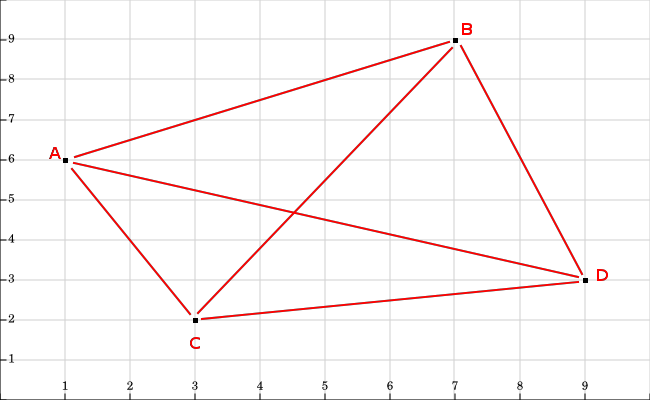
\includegraphics[scale=.50]{tsp2}
  \caption{Cities on a plane, displaying routes between pairs}
  \label{fig:tsp1}
\end{figure}

The travelling salesman problem is interesting in that the number of possible tours is the factorial of the size of the set of cities. For instance the example in \textit{Figure~\ref{fig:tsp1}} has 24 different tours. If a set of 12 cities is used there would be 479,001,600 tours \cite{tsp}.

This presents a problem with a massive search space and a well defined solution, that being the shortest tour. It also presents an opportunity to utilise a parallel algorithm which concurrently calculates the length of a tour; and determines if it is currently the shortest tour evaluated.

\subsubsection{Search Method}

With the travelling salesman being a search problem, there are a myriad of strategies which can be utilised in order to determine the shortest tour in the shortest possible amount of time \cite{tsp}.

In a test of raw language throughput however, the use of advanced searching algorithms and techniques would be superfluous at best. Therefore the computer programs produced will use a brute force approach; examining every possible tour and determining which is the shortest \cite{bruteForce}.

\subsubsection{Acceptance Tests}

In order to ensure that the programs produced correctly evaluate which tour is shortest for any given set of cities, a number of test cases with known results have been formulated.

Test cases are presented as a list of $x$ and $y$ co-ordinates as follows: 
\begin{displaymath}
[[1x,1y],[2x,2y],[3x,3y] \ldots [nx,ny]]
\end{displaymath}
\begin{enumerate}
  \item $[[1,1],[4,4],[7,7],[10,10]]$ \\ Shortest tour distance: 12.7279 \\ Tests that distances are calculated correctly when cities do not share either $x$ or $y$ co-ordinates.
    
  \item $[[1,1],[1,4],[5,5],[1,7]]$ \\ Shortest tour distance: 10.4721 \\ Tests that distances are calculated correctly when two or more cities share an $x$ co-ordinate.

  \item $[[1,1],[4,1],[6,6],[9,1]]$ \\ Shortest tour distance: 13.8309 \\ Tests that distances are calculated correctly when two or more cities share an $y$ co-ordinate.

  \item $[[1,1],[1,2],[1,5],[3,5],[7,5]]$ \\ Shortest tour distance: 10.0\\ Tests that distances are calculated correctly when multiple cities share either an $x$ or $y$ co-ordinate.

  \item $[[1,1],[4,4],[7,7],[10,10],[3,3],[6,6],[9,9],[2,2],[5,5],[8,8],[8,9],[5,7]]$
    \\ Shortest tour distance: 15.3137\\ A test with 12 cities and 479,001,600 possible tours. A stress test to ensure that the programs can cope with a large search space.
\end{enumerate}

It is expected that the aforementioned test cases will sufficiently exercise complete operation of the programs produced and ensure that results gathered are both complete and correct.

\newpage
\section{Design}

\subsection{Architecture}

The design of an application to satisfy the objectives of this paper will be completed in three stages.
\begin{enumerate} \itemsep0pt
  \item Firstly, a decision must be made regarding what is actually to be built. The objectives and features which must be satisfied have been well defined; however a question still remains regarding what will satisfy the test specification. 
  \item A set of tests will be developed in order to ensure that the computer program correctly addresses point 1. There must be no doubt that the program can successfully solve the problem in question.
  \item The computer program itself will be designed and implemented with rapid prototyping and iterative development.
\end{enumerate}

\subsection{Components}

Regardless of the language of implementation, a computer program designed to solve the travelling salesman problem will have distinct components. Hence the design of the program will attempt to remain as language agnostic as possible, with specific implementation details to be crystalized via rapid-prototyping. Individual components are discussed below, with a complete view of how they fit together displayed in \textit{Figure~\ref{fig:components}}
\begin{figure}[h]
  \centering
  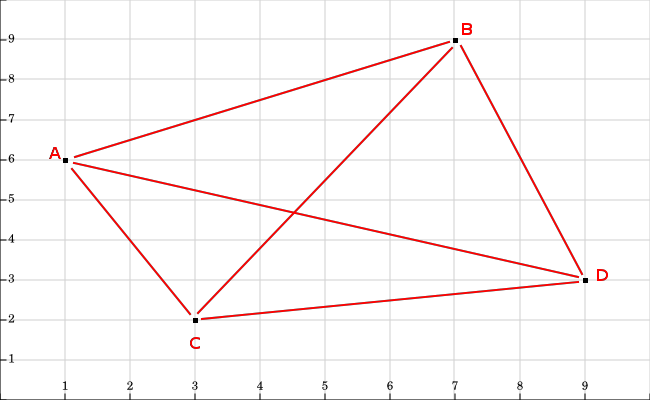
\includegraphics[scale=.50]{tsp2}
  \caption{Interaction between program components}
  \label{fig:components}
\end{figure}

\subsubsection{Run Controller}

The run controller is responsible for orchastrating the entire program. It is the primary controller and utilises all other components. Crucially, it is also responsible for recording the execution time of any given run. It should accept command line arguments regarding which set of cities to utilise, as well as how many runs are required.

\subsubsection{File Reader}

The file reader is responsible for taking a file of the form: x,y:x,y:x,y:x,y and converting it to a set of cities which the rest of the program can use to calculate the results with.

\subsubsection{Permutation Calculator}

Each individual tour is an ordered permutation of a set of cities. In order to evaluate all possible tours, there needs to be a facility by which a specific permutation can be generated.

\subsubsection{Distance Calculator}

Once a permutation has been obtained, its total distance must be calculated.

\subsubsection{Results Collector}

The results of each run, the time and shortest distance will be recorded in a data structure or structures, which can later be subjected to statistical analysis.

\subsubsection{Statistics Calculator}

This will contain a series of methods which are able to calculate both averages and standard deviations for the collected results.

\subsubsection{Results Printer}

Some mechanism is required to print the results to the screen or perhaps an output file.

\subsection{Flow of Control}

\section{Results}

\section{Conclusion}

\newpage
\singlespacing
\addcontentsline{roc}{section}{References}
\bibliographystyle{dcu}
\bibliography{bibliography}

\end{document}
